\documentclass[titlepage,a4paper,12pt]{ltjsreport}

\usepackage{luatexja}
\usepackage{amsmath,amsfonts}
\usepackage{amsthm}
\usepackage{bm}
\usepackage[dvipdfmx]{graphicx}
\usepackage{color}
\usepackage{caption}
\usepackage{url}
\usepackage{listings}
\usepackage{abstract}
\usepackage{multicol}
\usepackage{geometry}
\usepackage{here}


\lstset{
    basicstyle={\ttfamily},
    identifierstyle={\small},
    commentstyle={\small},
    keywordstyle={\small\bfseries},
    ndkeywordstyle={\small},
    stringstyle={\small\ttfamily},
    frame={tb},
    breaklines=true,
    columns=fixed,
    basewidth=0.465em,
    numbers=left,
    numberstyle={\scriptsize},
    lineskip=-0.5ex
}


\begin{document}

\leftline{課題5　要求記述}
\rightline{256E0143
三留 慎太郎}

\begin{enumerate}
    \item 概要 \mbox{}\\
    シンプソン公式を用いて、関数を数値積分する。

    \item 詳細\mbox{}\\
    関数として以下に示す式で表されるt分布を用いる。
    
    \[
    F(x) = \frac{ \Gamma\left( \frac{dof + 1}{2} \right) }
    { (dof \times \pi)^{\frac{1}{2}} \Gamma\left( \frac{dof}{2} \right) }
    \left( 1 + \frac{x^2}{dof} \right)^{- \frac{dof + 1}{2}}
    \]

    $\Gamma$はガンマ関数を表し、以下で表される。\\
    $\Gamma(x) = (x - 1)\Gamma(x - 1)$で、$\Gamma(1) = 1$, $\Gamma(\frac{1}{2}) = \sqrt{\pi}$\\
    
    ここで、$x$と$dof$を与え、範囲は0から$x$までの区間、自由度は$dof$とする。
    シンプソンの公式による積分の計算は以下の手順に沿って行う

    \begin{enumerate}
        \item $num\_seg = $セグメント数の初期値として、偶数値を与える。
        \item セグメントの幅$W = x/num\_seg$\\ 許容誤差範囲$E = 0.00001$
        \item 積分値を以下の計算式で計算する。
        
        \[
        p = \frac{W}{3} \left[ F(0) + \sum_{i=1,3,5\dots}^{\text{num\_seg}-1} 4F(iW) + \sum_{i=2,4,6\dots}^{\text{num\_seg}-2} 2F(iW) + F(x_i) \right]
        \]

        \item $num\_seg = 2 \times num\_seg$として再度積分値を計算する
        \item 二つの計算結果の値の差が$E$より大きい場合は$num\_seg$を2倍して再度積分値を計算し、差が$E$より小さくなるまで繰り返す。\\最後の結果を答えとする

    \end{enumerate}


    \item 入力\mbox{}\\
    
    \begin{itemize}
        \item データの入力：csvファイル入力
        \item 入力ファイル：図\ref{data}のように、カンマ区切りの表形式で表現し、$x$,$dof$を持つ。\\
        
        \begin{figure}[H]
            \centering
            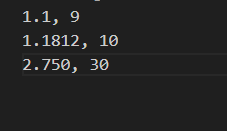
\includegraphics[width=0.4\textwidth]{../picture/課題5/data.png}
            \caption{入力データ}
            \label{data}
        \end{figure}
        
        \item 実行時の入力：コマンドラインに以下の形式で入力
        　java プログラム名 実数値入力ファイル名 用いるデータの列番号1 用いるデータの列番号2 
        \item 実行時入力例：java Program5 data\_program5.csv 1 2\\
                
    \end{itemize}


    \item 出力\mbox{}\\
    \begin{itemize}
        \item 出力方法：コマンドライン出力
        \item 出力する値：入力データすべての行に対応する積分値
        \item 精度：少数点以下第6位を四捨五入して表示する。
        \item 出力例：図\ref{kitaiti}のように出力する値をそれぞれ改行して表示する。
        
        \begin{figure}[H]
            \centering
            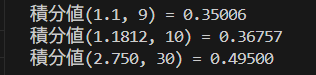
\includegraphics[width=0.4\textwidth]{../picture/課題5/kitaiti.png}
            \caption{出力例}
            \label{kitaiti}
        \end{figure}

    \end{itemize}


    \item テスト\mbox{}\\
    図\ref{testdata}のデータを用いてテストを行う。
    期待値を図\ref{testkitaiti}に示す。

    \begin{figure}[H]
        \centering
        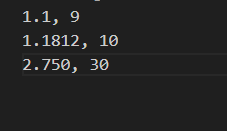
\includegraphics[width=0.4\textwidth]{../picture/課題5/testdata.png}
        \caption{テストデータ}
        \label{testdata}
    \end{figure}

    \begin{figure}[H]
        \centering
        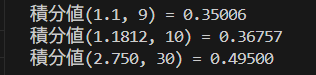
\includegraphics[width=0.4\textwidth]{../picture/課題5/testkitaiti.png}
        \caption{期待値}
        \label{testkitaiti}
    \end{figure}

     

\end{enumerate}



\end{document}